\pagestyle{fancy}
\renewcommand{\theUnit}{6}
\ifthenelse{\isundefined{\UnitPageNumbers}}{}{\setcounter{page}{1}}
\rhead{Chapter \theUnit: Estimation}
\lhead{Math 3382: Statistical Theory}
%\lhead{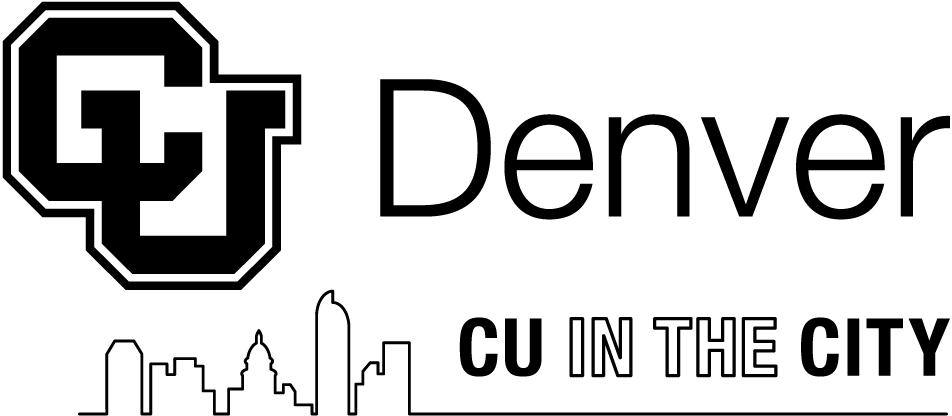
\includegraphics[width=1.25cm]{CUDenver-Logo.png}}
\rfoot{\mypage}
\cfoot{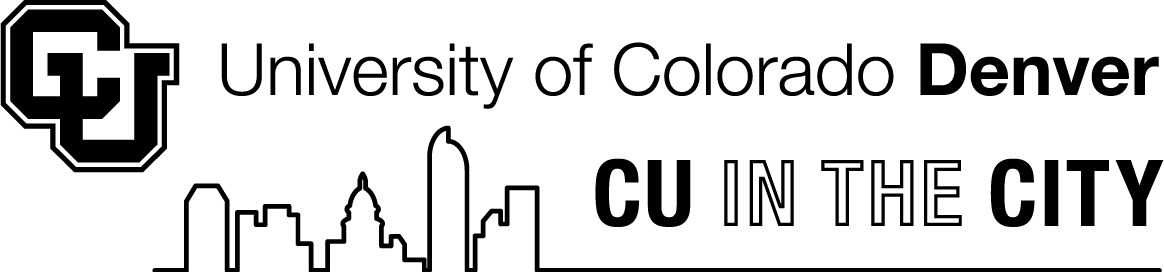
\includegraphics[width=2.25cm]{CUDenver-Logo-coverpage.png}}
\lfoot{Adam Spiegler}
\fancypagestyle{firstfooter}{\footskip = 50pt}
\renewcommand{\footrulewidth}{.4pt}
%%%%%%%%%%%%%%%%%%%%%%%%%%%
\vspace*{-20pt} \thispagestyle{firstfooter}


%\begin{tasks}[counter-format = {(tsk[a])},label-offset = {0.8em},label-format = {\color{black}\bfseries}](2)


\pagebegin{Section 6.2: Method of Moments (MOM) Estimates}


\bi
\ii Let $X$ be a random variable with pdf $f(x; \theta_1, \theta_2, \ \ldots \theta_k)$ that depends on parameters $\theta_1, \theta_2, \ldots , \theta_k$. \medskip

\ii If we independently pick a random variables $X_1, X_2, \ldots X_n$ from population $X$, we can determine what values of $\theta_1, \theta_2, \ldots , \theta_k$  that best fit the data in the following sense:

\bb
\ii The mean of the population $X$ equals the sample mean.
\ii The variance of the population equals the variance of the sample.
\ii The skewness of the population equals the skewness of the sample.
\ii $\ldots$ and so on.
\ee

\ii We find values of the parameters so the properties of random variable $X$ are equal to corresponding properties of our sample.
  \ei


  \bbox
Let $X$ be a random variable with pdf $f(x)$. For a positive integer $k$, \colorb{\textbf{the kth theoretical moment of $X$}} is
\[ \mu_k = E \lbrack X^k \rbrack = \int_{-\infty}^{\infty} x^kf(x) \, dx \ \ \ \mbox{ or } \ \ \  \mu_k = E\lbrack X^k \rbrack = \sum_X x^kf(x),\]


\begin{multicols}{2}

\bi
  \ii The \colorr{mean} $\mu = E \lbrack X \rbrack$ is the first moment. 
  \ii The \colorr{variance} is related to the second moment $\mu_2 = E \lbrack X^2 \rbrack$.
  \ii The \colorr{skewness} is related the third moment $\mu_3 = E \lbrack X^3 \rbrack$.
  \ii The \colorr{kurtosis} (how ``peaky'' or flat the distribution is) is related to $\mu_4 = E \lbrack X^4 \rbrack$.
  \ei

\columnbreak

\begin{center}
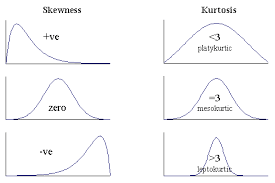
\includegraphics[width=0.5\tw]{15/fig-moments.png}
\end{center}

\end{multicols}

For a sample we called the corresponding properties \colorb{\textbf{sample moments}} denoted by \colorb{$M_k$}.

\ebox


\clearpage

%\bbox
%Let $X$ be a random variable with mean $\mu$. The \textbf{skewness} of $X$ measure how symmetric the distribution of $X$ is. The skewness can be found using the third central moment, $\mu_3$:
%\[ \mbox{Skewness} =  \frac{E \lbrack (X-\mu)^3 \rbrack}{\sigma^3} = \frac{\mu_3}{\sigma^3}.\]
%\bi
%\ii If a distribution is symmetric, its skewness is zero.
%\ii If a distribution is skewed to the right, its skewness is positive.
%\ii If a distribution is skewed to the left, its skewness is negative.
%\ei
%\ebox

%\bbox
%Let $X$ be a random variable with mean $\mu$. Informally, the \textbf{kurtosis} of $X$ measures how ``peaky'' or flat  the distribution of $X$ is. The skewness can be found using the fourth central moment $\mu_4$:\footnote{Subtracting three actually gives the excess kurtosis. This is often done so the kurtosis of a normal distribution is equal to 0. In some texts, the $-3$ is not included, in which case a normal distribution has kurtosis equal to 3.}
%\[ \mbox{Kurtosis} =  \frac{E \lbrack (X-\mu)^4 \rbrack}{\sigma^4} = \frac{\mu_4}{\sigma^4} -3.\]
%\bi
%\ii If the kurtosis is zero, then the distribution is peaked like a normal distribution.
%\ii If the kurtosis is positive, then the distribution is more peaked than a normal distribution.
%\ii If the kurtosis is negative, then the distribution is flatter than a normal distribution.
%\ei
%\ebox


\pagebegin{Section 6.2: Method of Moments Estimate}

  \bb
  \ii Let $X$ be a random variable with pdf $\dsty f(x; \lambda, \delta)=\lambda e^{-\lambda(x-\delta)}$ for $x > \delta$ with parameters $\lambda, \delta >0$. Find the first and second theoretical moments of $X$.  \vfill

  
\ii Let $X_1=3$, $X_2=4$, $X_3 = 5$, and $X_4 = 8$ be a random sample from a random variable $X$ with pdf $f(x; \lambda, \delta)$. Find the first and second sample moments. \label{sample} \vfill
\ee


\bbox
Let $X$ be a random variable with pdf $f(x; \theta_1, \theta_2, \ldots, \theta_k)$ and let $X_1$, $X_2$, $\ldots$, $X_n$ be a random
sample.
\bi
\ii The theoretical moments $\mu_k$ are functions of the $k$ parameters $\theta_1, \theta_2, \ldots, \theta_k$.
\ii The sample moments $M_k$ are values we calculate based on the sample.
\ii The \alert{method of moments (MOM) estimate} is obtained by solving the system:
\ei

\begin{align*}
\mu_1 = \int_{-\infty}^{\infty} xf(x) \, dx &= \frac{1}{n} \sum_{i=1}^n X_i = M_1\\
\mu_2 = \int_{-\infty}^{\infty} x^2f(x) \, dx &= \frac{1}{n} \sum_{i=1}^n X_i^2 = M_2\\
& \vdots \\
\mu_k = \int_{-\infty}^{\infty} x^kf(x) \, dx &= \frac{1}{n} \sum_{i=1}^n X_i^k = M_k
\end{align*}

If $X$ is a discrete random variable, change the integrals to summations.
\ebox

\clearpage

\pagebegin{Practice}
  
\bb[resume]
\ii Let $X$ be a random variable with pdf $\dsty f(x; \lambda, \delta)=\lambda e^{-\lambda(x-\delta)}$ for $x > \delta$ with parameters $\lambda, \delta >0$. If $X_1=3$, $X_2=4$, $X_3 = 5$, and $X_4 = 8$ is a random sample picked from random variable $X$, find the first and second sample moments. \label{sample} \vfill

\ii Let $X_1=1, X_2=3, X_3=7, X_4=10$ be four numbers picked at random from the uniform distribution on $\lbrack \alpha , \beta \rbrack$. Find the MoM estimates of $\alpha$ and $\beta$. \vfill

\ee

\clearpage


\pagebegin{Section 6.3.1: Unbiasedness}

  \alert{Which method is best?} We will wrap up Chapter 6 by looking at some properties we can use to gauge estimates, such as unbiasedness, efficiency, and Mean Square Error. \medskip

\bbox
  \alert{Bias:} We like an estimator to be, on average,  equal to the parameter it is estimating: $E \lbrack \hat{\theta} \rbrack -\theta =0$.
  \bi
  \ii Sample mean is unbiased estimator of $\mu$.
  \ii Sample proportion is an unbiased estimator of $p$.
 % \ii The MLE estimate for $\sigma^2$, $\hat{\sigma}^2$, is biased.
  \ei

%In practice, we are satisfied when estimates are approximately unbiased. Estimates that are exactly unbiased may be impossible or unreasonable at times.
\ebox

\bb[resume]
\ii Show that the MLE estimate for the variance for $X \sim N(\mu, \sigma^2)$,
  \[ \hat{\sigma}^2 =\frac{1}{n} \sum_{i=1}^n (x_i-\bar{x})^2,\]
  is a biased estimate for  $\sigma^2$
\ee

  \vspace{3in}

%In practice, we are satisfied when estimates are approximately unbiased. Estimates that are exactly unbiased may be impossible or unreasonable at times (maybe probability example or sample standard deviation?).

\clearpage


\pagebegin{Section 6.3.2: Efficiency}

  Let $X_1, X_2, X_3$ be independent random variables from an identical distribution with mean and variance $\mu$ and $\sigma^2$, respectively.

  \bi
  \ii We have shown $\dsty \bar{X} = \frac{X_1+X_2+X_3}{3}$ is an unbiased estimator of $\mu$.
  \ii The weighted mean $\dsty Y = \frac{1}{6}X_1 + \frac{1}{3}X_2 + \frac{1}{2}X_3$ is also unbiased.
  \ii Is one better than the other?
  \ei

  
\bb[resume]
\ii We have two unbiased estimators of $\mu$ given below.  Which estimator has less variability?
  \[ \bar{X} = \frac{X_1+X_2+X_3}{3} \ \ \ \mbox{and} \ \ \ Y = \frac{1}{6}X_1 + \frac{1}{3}X_2 + \frac{1}{2}X_3.\]

\ms

 \colorg{ \[ \Var \lbrack \bar{X} \rbrack = \Var \left[ \frac{X_1+X_2+X_3}{3} \right] = \frac{1}{3^2} (3 \sigma^2)= \frac{\sigma^2}{3} .\] }

\ms

 \colorr{  \[ \Var \lbrack Y \rbrack = \Var \left[ \frac{1}{6}X_1 + \frac{1}{3}X_2 + \frac{1}{2}X_3 \right] =\left( \frac{1}{36}+ \frac{1}{9}+\frac{1}{4} \right)(3 \sigma^2) = \frac{7}{18} \sigma^2.\] }

\ms
\ee

  
  \bbox
    If $\theta_1$ and $\theta_2$ are both unbiased estimators of $\theta$, then  $\theta_1$ is said to be
    more \alert{efficient} than $\theta_2$ if $\Var \lbrack \theta_1 \rbrack < \Var \lbrack \theta_2 \rbrack$.
  \ebox

\pagebegin{Section 6.3.3: Mean Square Error}

 \bbox
   The \alert{Mean Square Error (MSE)} of an estimator measures the average squared distance between the estimator and the parameter:
 \[ \mbox{MSE} \lbrack \hat{\theta} \rbrack = \Exp \lbrack (\hat{\theta}-\theta)^2 \rbrack.\]


 \alert{Proposition 6.3.3} shows that  $\mbox{MSE} \lbrack \hat{\theta} \rbrack = \Var  \lbrack \hat{\theta} \rbrack + (\mbox{Bias} \lbrack \hat{\theta} \rbrack)^2$.
\ebox

 \bi
 \ii MSE is  a criterion that  combines bias and variance.
\ii If two estimators are unbiased, one is more efficient than the other if and only if its MSE is smaller.
\ii In general, we are often faced with a trade-off between variability and bias.
\ei


\clearpage


 \bb[resume]
\ii Let $X \sim \mbox{Binom}(n,p)$ with $n$ known and parameter $p$ unknown.
  \bb
  \ii Find the variance and MSE for if we use the sample proportion $\hat{p}_1 = \frac{X}{n}$ as an estimate for $p$. \vfill
%  \[ \Var \left[ \hat{p}_1 \right] = \frac{p(1-p)}{n} \ \ \ \mbox{and} \ \ \ \mbox{MSE} \left[ \hat{p}_1 \right] =  \frac{p(1-p)}{n} .\]
  \ii If we add two more trials to the sample, and assume one is a failure and the other a success, then we can define a second estimator for $p$
  \[ \hat{p}_2 = \frac{X+1}{n+2}. \] \vfill
  \ii Is $\hat{p}_2$ is a biased or unbiased estimator for $p$? \vfill
  %since $E \left[ \hat{p}_2 \right] = \frac{np+1}{n+2}$ which gives
%  \[ \mbox{Bias}\left[ \hat{p}_2 \right] = \frac{np+1}{n+2} - p = \frac{1-2p}{n+2}.\]
   \ii Find the $\Var \left[ \hat{p}_2 \right]$ and $\mbox{MSE} \left[ \hat{p}_2 \right]$. \vspace{2.5in}
   \ee
\ee

\hspace{4in}    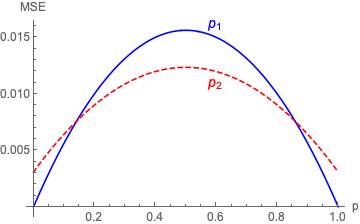
\includegraphics[width=2.5in]{15/chap6-mse.png}


\bbox
    \bi
    \ii We have looked at two more estimators for unknown population parameters: MLE and MoM.
    \ii We looked at different criteria to compare different estimators: Bias, Efficiency, and MSE.
    \ii The text discusses more properties at the end of Section 6.3 that are more technical.
    \ei
  \ebox  




 
